El sistema consiste en un proceso central llamado \emph{maestro}, un n�mero variable de procesos en diferentes computadores de una red llamados \emph{esclavos} y un n�mero de procesos \emph{cliente} que generan tareas agrupadas en trabajos. En la figura \ref{fig:image01} se grafica este esquema.
\begin{figure}
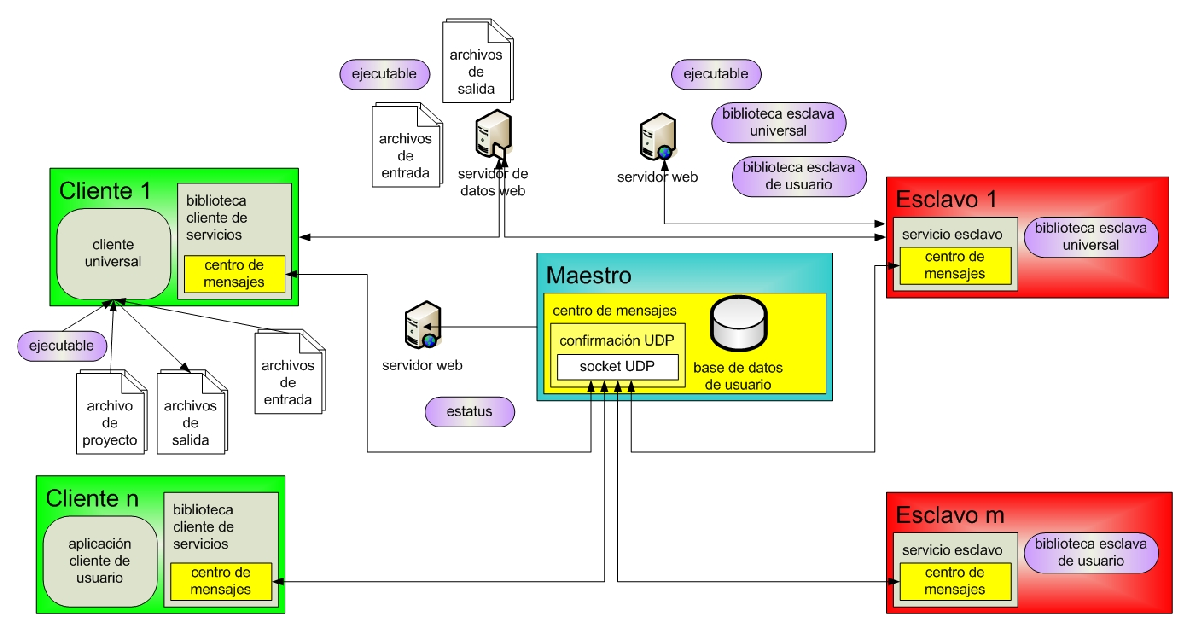
\includegraphics[width=\textwidth]{images/image01.eps}
\caption{La arquitectura de Q$^2$ADPZ}
\label{fig:image01}
\end{figure}
El componente esclavo corre como un proceso permanente. Su rol principal es notificar al \emph{maestro} sobre su estado y sus recursos disponibles. Otro rol que posee es lanzar una aplicaci�n, consecuencia de una petici�n del maestro. La aplicaci�n, en la forma de una biblioteca, ejecutable o programa interpretado, es transferida desde el servidor de acuerdo a la descripci�n de la tarea, entonces es ejecutada con los argumentos de l�nea de comando especificadas en dicha descripci�n.

Al momento en que un esclavo recibe una tarea, en primera instancia descarga el ejecutable o programa interpretado desde un repositorio autom�tico de datos (implementado sobre un servidor web en Perl), o desde una direcci�n URL. Luego, el esclavo procede a descargar y preparar todos los archivos de entrada requeridos. Despu�s que el ejecutable o programa interpretado termina, los archivos de salida generados son subidos al repositorio web para ser posteriormente obtenidos por el cliente que cre� la tarea.

El maestro adem�s escucha a todos los esclavos y de esta forma tiene una visi�n general de todos los recursos disponibles en el sistema. El maestro acepta peticiones de tareas de los clientes y le asigna los nodos (esclavos) m�s adecuados. Adem�s de esto, el maestro permite reservar nodos: los clientes son notificados despu�s de que los recursos se encuentren disponibles.

El cliente consiste en una aplicaci�n que usa una biblioteca cliente de servicios. Esta biblioteca provee una API C++ para la comunicaci�n con el maestro, permitiendo controlar y comenzar trabajos y tareas, adem�s de obtener los resultados de �stos. Los usuarios pueden utilizar la API directamente en sus aplicaciones o usar un cliente universal que ingresa y controla las tareas en base a un archivo de especificaci�n en formato XML.
